%\appendix

\begin{widetext}

\section{Flow equations}
\label{sec:FlowEquations}

Here we present the final expressions for the flow equations in the pairing and in the charge channels. The flow equations for the magnetic channel have been presented in
Sec.~\ref{sec:vertex}.

The flow equation for the $s$-wave pairing channel reads
\begin{equation}
\dot{\mathcal{S}}_{\bs{Q},\Omega}(\nu_1,\nu_3) = 
  \frac{1}{2} \sum_\nu L^{\mathrm{s},\Lambda}_{\mathbf{Q},\Omega}(\nu_1,\nu) P^{\mathrm{s},\Lambda}_{\bs{Q},\Omega}(\nu)
  L^{\mathrm{s},\Lambda}_{\mathbf{Q},\Omega}(\nu,\Omega-\nu_3) +
 \frac{1}{2} \sum_\nu L^{\mathrm{s},\Lambda}_{\mathbf{Q},\Omega}(\Omega-\nu_1,\nu)
 P^{\mathrm{s},\Lambda}_{\bs{Q},\Omega}(\nu)
 L^{\mathrm{s},\Lambda}_{\mathbf{Q},\Omega}(\nu,\nu_3),
\end{equation}  
with
\begin{equation}
 P^{\mathrm{s},\Lambda}_{\bs{Q},\Omega}(\omega) = \int_{\bs{p}}
 G^{\Lambda}(\bs{p},\omega)S^{\Lambda}(\bs{Q}-\bs{p},\Omega-\omega) +
 G^{\Lambda}(\bs{Q}-\bs{p},\Omega-\omega) S^{\Lambda}(\bs{p},\omega), 
\label{eq:app:P_pp}
\end{equation} 
and
\begin{align} 
\label{eq:Lswave}
 L^{\mathrm{s},\Lambda}_{\mathbf{Q},\Omega}(\nu_1,\nu_3) = U-\mathcal{S}^{\Lambda}_{\bs{Q},\Omega} (\nu_1,\nu_3) +
 \int_{\bs{p}} \Big[ \mathcal{M}^{\Lambda}_{\bs{p},\nu_3-\nu_1}(\nu_1,\Omega-\nu_1) + \frac{1}{2} \mathcal{M}^{\Lambda}_{\bs{p},\Omega-\nu_1-\nu_3}(\nu_1,\Omega-\nu_1) -
 \frac{1}{2} \mathcal{C}^{\Lambda}_{\bs{p},\Omega-\nu_1-\nu_3}(\nu_1,\Omega-\nu_1) \Big]. 
\end{align}	 
The flow equation for the $d$-wave pairing channel reads
\begin{equation}
 \dot{\mathcal{D}}^{\Lambda}_{\bs{Q},\Omega}(\nu_1,\nu_3) = 
 \frac{1}{2} \sum_\nu L^{\mathrm{d},\Lambda}_{\bs{Q},\Omega}(\nu_1,\nu)
 P^{\mathrm{d},\Lambda}_{\bs{Q},\Omega(\nu)}
 L^{\mathrm{d},\Lambda}_{\bs{Q},\Omega} (\nu,\Omega-\nu_3) + 
 \frac{1}{2} \sum_\nu L^{\mathrm{d},\Lambda}_{\bs{Q},\Omega}(\Omega-\nu_1,\nu)
 P^{\mathrm{d},\Lambda}_{\bs{Q},\Omega}(\nu)
 L^{\mathrm{d},\Lambda}_{\bs{Q},\Omega}(\nu,\nu_3),
\label{eq:dwaveflow}
\end{equation}
with
\begin{equation}
 P^{\mathrm{d},\Lambda}_{\bs{Q},\Omega}(\omega) =
 \int_{\bs{p}} \left[ f_{\mathrm{d}}\left( \bs{Q}/2 - \bs{p} \right) \right]^2 
\left[ G^{\Lambda}(\bs{p},\omega)S^{\Lambda}(\bs{Q}-\bs{p},\Omega-\omega) +G^{\Lambda}(\bs{Q}-\bs{p},\Omega-\omega)
S^{\Lambda}(\bs{p},\omega) \right], 
\label{eq:app:P_pp}
\end{equation} 
and
\begin{align} 
\label{eq:Ldwave}
 L^{\mathrm{d},\Lambda}_{\bs{Q},\Omega}(\nu_1,\nu_3) =
 -\mathcal{D}^{\Lambda}_{\bs{Q},\Omega}(\nu_1,\nu_3)
 + \frac{1}{2}\int_{\bs{p}} \left(\cos{p_x}+\cos{p_y}\right) \Big[ 
 & \mathcal{M}^{\Lambda}_{\bs{p},\nu_3-\nu_1}(\nu_1,\Omega-\nu_1) 
 + \frac{1}{2} \mathcal{M}^{\Lambda}_{\bs{p},\Omega-\nu_1-\nu_3}(\nu_1,\Omega-\nu_1)
 \\ \nonumber
 & - \frac{1}{2} \mathcal{C}^{\Lambda}_{\bs{p},\Omega-\nu_1-\nu_3}(\nu_1,\Omega-\nu_1) \Big].
\end{align} 
Since $\mathcal{D}$ is generated exclusively by fluctuation contributions (not by the bare $U$), see Eq. (\ref{eq:Ldwave}), it is the most sensitive channel to approximations on the frequency dependence.  
Neglecting the frequency dependence of the vertex one likely overestimates $L^d{\mathrm{d}}$, as already mentioned in Ref.~\onlinecite{Husemann2012}.

The flow equation for the charge channel reads
\begin{equation}
\dot{\mathcal{C}}^{\Lambda}_\bs{Q,\Omega}(\nu_1,\nu_2) = \sum_\nu
 L^{\mathrm{c},\Lambda}_{\bs{Q},\Omega}(\nu_1,\nu) P^{\Lambda}_{\bs{Q},\Omega}(\nu) 
 L^{\mathrm{c},\Lambda}_{\bs{Q},\Omega}(\nu,\nu_2-\Omega), 
\end{equation} 	   
with $P^{\Lambda}_{\bs{Q},\Omega}(\omega)$ as in Eq.~(\ref{eq:Pph}), and
\begin{align}  
 L^{\mathrm{c},\Lambda}_{\bs{Q},\Omega}(\nu_1,\nu_2) & =
 U - \mathcal{C}^{\Lambda}_{\bs{Q},\Omega}(\nu_1,\nu_2)
 + \int_{\bs{p}} \Big [
 - 2 \mathcal{S}^{\Lambda}_{\bs{p},\nu_1+\nu_2}(\nu_1,\nu_2-\Omega) + \mathcal{S}^{\Lambda}_{\bs{p},\nu_1+\nu_2}(\nu_1,\Omega+\nu_1)
 \nonumber \\ 
 & +  [\cos(Q_x)+\cos(Q_y)]\left( \mathcal{D}^{\Lambda}_{\bs{p},\nu_1+\nu_2}(\nu_1,\nu_2-\Omega) -\frac{1}{2} \mathcal{D}^{\Lambda}_{\bs{p},\nu_1+\nu_2}(\nu_1,\Omega+\nu_1) \right)
 \nonumber \\
 & + \frac{3}{2} \mathcal{M}^{\Lambda}_{\bs{p},\nu_2-\nu_1-\Omega}(\nu_1,\nu_2)
 + \frac{1}{2} \mathcal{C}_{\bs{p},\nu_2-\nu_1-\Omega}(\nu_1,\nu_2) \Big] .
 \label{eq:Lc}
\end{align}
The equation for the magnetic channel is reported in Eq. (\ref{eq:FlowMag}).
The form factor decomposition allows to decouple the momentum integrals, in the calculation of the $L$'s, Eqs.~(\ref{eq:Lxph}), (\ref{eq:Lswave}), (\ref{eq:Ldwave}) and (\ref{eq:Lc}), from the frequency summations in the flow equations, hence reducing the numerical effort.   	 

\section{Pairing channel}
\label{sec:appPairingChannel}

\begin{figure}[tbh]
 % \begin{center}
    \subfigure[$x=0.025$]{
    \label{fig:pairing975}
    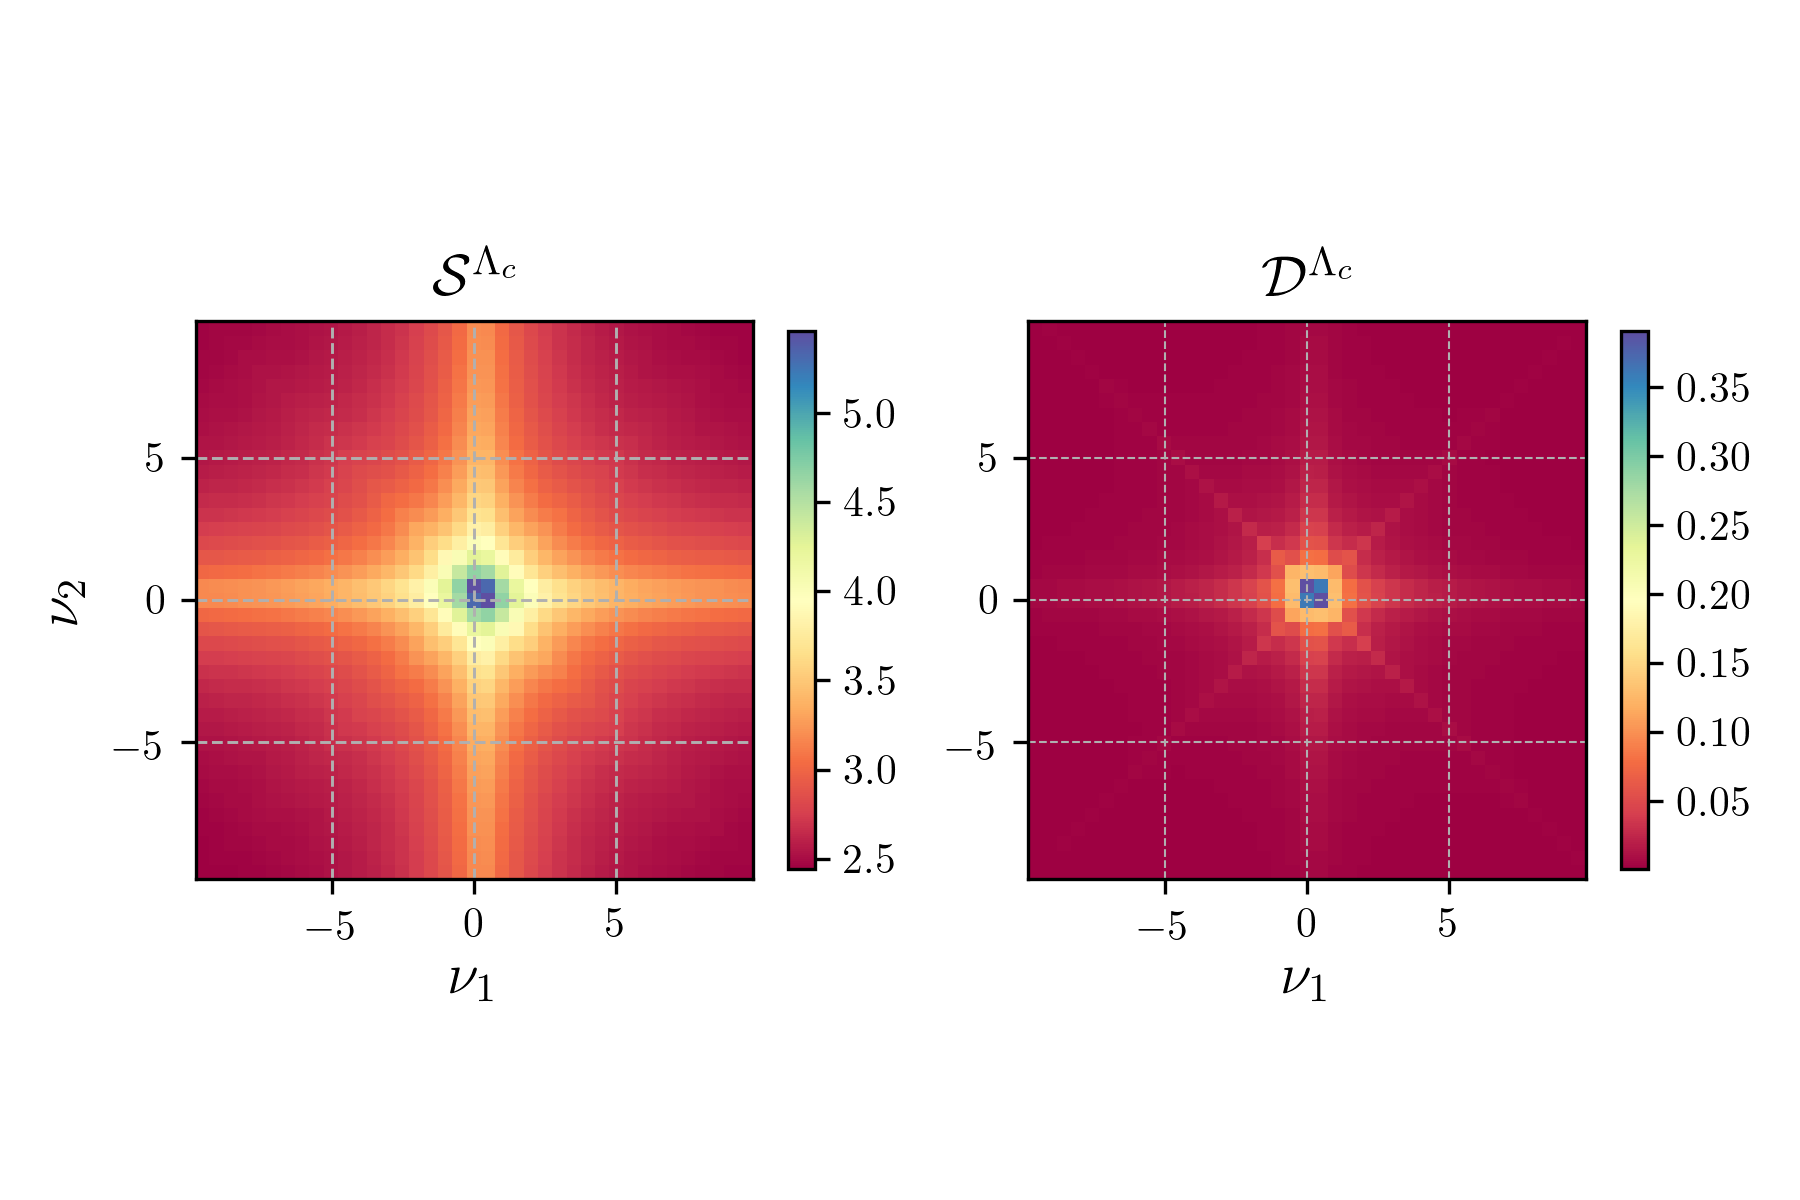
\includegraphics[scale=0.55]{images/Phi_color_s_d_wave_SE_fill0_975.png}}
    \subfigure[$x=0.4$]
    {
    \label{fig:pairing600}
    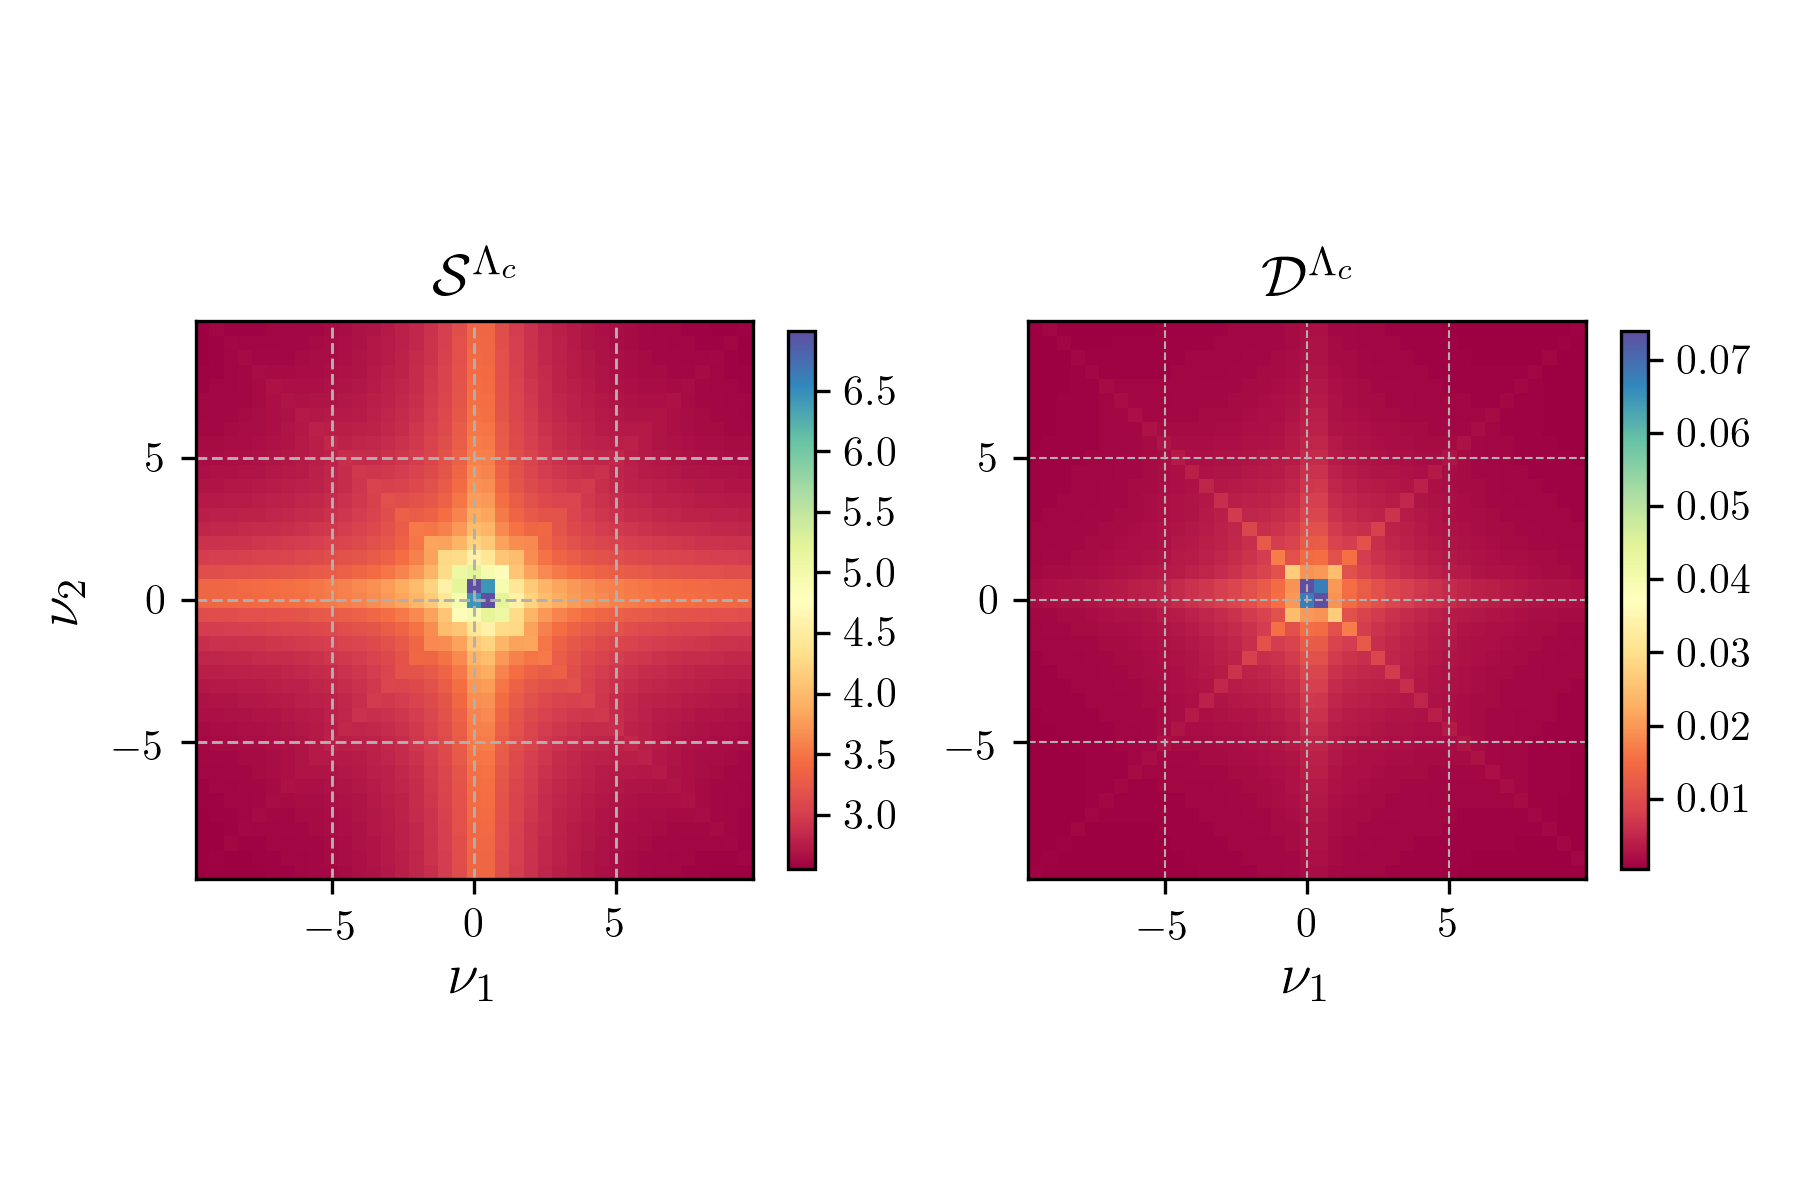
\includegraphics[scale=0.55]{images/Phi_color_s_d_wave_SE_fill0_600.png}} 
 % \end{center}
\caption{Frequency dependence of the pairing channels
 $\mathcal{S}^{\Lambda_c}_{\bs{Q},\Omega}(\nu_1,\nu_2)$ and
 $\mathcal{D}^{\Lambda_c}_{\bs{Q},\Omega}(\nu_1,\nu_2)$ for $\bs{Q}=(0,0)$ and $\Omega=0$.
 The doping is $x=0.025$ (left) and $x=0.4$ (right). The other parameters are $T=0.08t$, $t'=-0.32t$, and $U=4t$.}
\label{fig:pairing}
\end{figure}

In Fig.~\ref{fig:pairing} we display the frequency dependence of the pairing functions $\mathcal{S}$ and $\mathcal{D}$ for two distinct doping values $x=0.025$ and $x=0.4$. 
As a consequence of Eq.~(\ref{eq:Ldwave}), $\mathcal{D}^{\Lambda_c}$ is decaying to zero in all directions for increasing $|\nu_1|$, $\nu_2|$.\cite{Wentzell2016a}
The small numerical values of $\mathcal{D}^{\Lambda_c}$ are due to three main reasons: 
first, the $d$-wave pairing is expected to increase suddenly only for temperatures very close to its critical temperature. 
Second, as argued in Ref.~\onlinecite{Husemann2012}, previous fRG calculations with a static vertex overestimate the $d$-wave channel by neglecting the frequency dependence in Eq.~(\ref{eq:Ldwave}). 
Finally, the interaction scheme itself has a tendency to suppress the $d$-wave pairing. 
This can be understood considering the diagrams that contribute to the $d$-wave channel. In fact, unlike the other channels, $\mathcal{D}$ is generated by diagrams containing at least \emph{two} overlapping loops, sharing some of the loop arguments. This kind of diagrams is underestimated by a multiplicative regulator, like in the interaction scheme.  
This is explained in detail in Section V~2 of Ref.~\onlinecite{Wentzell2016a}.

\end{widetext}